%\documentclass[opre,blindrev]{informs3}
\documentclass[opre,nonblindrev]{informs3} % current default for manuscript submission

%%\DoubleSpacedXI % Made default 4/4/2014 at request
\OneAndAHalfSpacedXI % current default line spacing
%%\OneAndAHalfSpacedXII
%%\DoubleSpacedXII
%%\SingleSpacedXI
%%\SingleSpacedXII

% If hyperref is used, dvi-to-ps driver of choice must be declared as
%   an additional option to the \documentclass. For example
%\documentclass[dvips,opre]{informs3}      % if dvips is used
%\documentclass[dvipsone,opre]{informs3}   % if dvipsone is used, etc.

%%% OPRE uses endnotes. If you do not use them, put a percent sign before
%%% the \theendnotes command. This template does show how to use them.
% \usepackage{endnotes}
% \let\footnote=\endnote
% \let\enotesize=\normalsize
% \def\notesname{Endnotes}%
% \def\makeenmark{$^{\theenmark}$}
% \def\enoteformat{\rightskip0pt\leftskip0pt\parindent=1.75em
%   \leavevmode\llap{\theenmark.\enskip}}

% Private macros here (check that there is no clash with the style)

% Natbib setup for author-year style
\usepackage{natbib}
 \bibpunct[, ]{(}{)}{,}{a}{}{,}%
 \def\bibfont{\small}%
 \def\bibsep{\smallskipamount}%
 \def\bibhang{24pt}%
 \def\newblock{\ }%
 \def\BIBand{and}%

\usepackage{bbm}
\usepackage{amsmath,amssymb,mathtools}
\usepackage{caption}
\usepackage{algorithmic}

\newcommand{\Prob}{\mathbb{P}}
\newcommand{\E}{\mathbb{E}}
\newcommand{\EI}{\mathrm{EI}}
\newcommand{\Dir}{\mathrm{Dirichlet}}
\newcommand{\PI}{\text{P}^*}
\newcommand{\mb}{\mathbf}
\newtheorem{Algorithm}{Algorithm}

%% Setup of theorem styles. Outcomment only one.
%% Preferred default is the first option.
\TheoremsNumberedThrough     % Preferred (Theorem 1, Lemma 1, Theorem 2)
%\TheoremsNumberedByChapter  % (Theorem 1.1, Lema 1.1, Theorem 1.2)
\ECRepeatTheorems

%% Setup of the equation numbering system. Outcomment only one.
%% Preferred default is the first option.
\EquationsNumberedThrough    % Default: (1), (2), ...
%\EquationsNumberedBySection % (1.1), (1.2), ...

% In the reviewing and copyediting stage enter the manuscript number.
%\MANUSCRIPTNO{} % When the article is logged in and DOI assigned to it,
                 %   this manuscript number is no longer necessary

%%%%%%%%%%%%%%%%
\begin{document}
%%%%%%%%%%%%%%%%

% Outcomment only when entries are known. Otherwise leave as is and
%   default values will be used.
%\setcounter{page}{1}
%\VOLUME{00}%
%\NO{0}%
%\MONTH{Xxxxx}% (month or a similar seasonal id)
%\YEAR{0000}% e.g., 2005
%\FIRSTPAGE{000}%
%\LASTPAGE{000}%
%\SHORTYEAR{00}% shortened year (two-digit)
%\ISSUE{0000} %
%\LONGFIRSTPAGE{0001} %
%\DOI{10.1287/xxxx.0000.0000}%

% Author's names for the running heads
% Sample depending on the number of authors;
% \RUNAUTHOR{Jones}
% \RUNAUTHOR{Jones and Wilson}
% \RUNAUTHOR{Jones, Miller, and Wilson}
% \RUNAUTHOR{Jones et al.} % for four or more authors
% Enter authors following the given pattern:
\RUNAUTHOR{Jialei, Pu and Peter}

% Title or shortened title suitable for running heads. Sample:
% \RUNTITLE{Bundling Information Goods of Decreasing Value}
% Enter the (shortened) title:
\RUNTITLE{Bayesian Active Learning for Finding Maximally-valued Exemplars}

% Full title. Sample:
% \TITLE{Bundling Information Goods of Decreasing Value}
% Enter the full title:
\TITLE{Bayesian Active Learning for Finding Maximally-valued Exemplars}

% Block of authors and their affiliations starts here:
% NOTE: Authors with same affiliation, if the order of authors allows,
%   should be entered in ONE field, separated by a comma.
%   \EMAIL field can be repeated if more than one author
\ARTICLEAUTHORS{%
\AUTHOR{Jialei Wang}
\AFF{School of Operations Research \& Information Engineering, Cornell University, Ithaca, NY 14853, \EMAIL{jw865@cornell.edu}} %, \URL{}}
\AUTHOR{Pu Yang}
\AFF{School of Operations Research \& Information Engineering, Cornell University, Ithaca, NY 14853, \EMAIL{py75@cornell.edu}} %, \URL{}}
\AUTHOR{Peter I. Frazier}
\AFF{School of Operations Research \& Information Engineering, Cornell University, Ithaca, NY 14853, \EMAIL{pf98@cornell.edu}} %, \URL{}}
% Enter all authors
} % end of the block

\ABSTRACT{%
We consider a Bayesian optimal search problem, related to active learning and arising in an application to materials science. In active learning, we have training data with unknown binary labels. Obtaining labels is expensive, and we wish to obtain a small number of labels, so that the statistical classifier built from them is good. We consider a variant in which each datapoint has an associated known value, and our goal is to find a datapoint with a positive label and large value.
% Enter your abstract
}%

% Sample
%\KEYWORDS{deterministic inventory theory; infinite linear programming duality;
%  existence of optimal policies; semi-Markov decision process; cyclic schedule}

% Fill in data. If unknown, outcomment the field
% \KEYWORDS{Bayesian, Active Learning, Naive Bayes} 

\maketitle
%%%%%%%%%%%%%%%%%%%%%%%%%%%%%%%%%%%%%%%%%%%%%%%%%%%%%%%%%%%%%%%%%%%%%%

% Samples of sectioning (and labeling) in OPRE
% NOTE: (1) \section and \subsection do NOT end with a period
%       (2) \subsubsection and lower need end punctuation
%       (3) capitalization is as shown (title style).
%
%\section{Introduction.}\label{intro} %%1.
%\subsection{Duality and the Classical EOQ Problem.}\label{class-EOQ} %% 1.1.
%\subsection{Outline.}\label{outline1} %% 1.2.
%\subsubsection{Cyclic Schedules for the General Deterministic SMDP.}
%  \label{cyclic-schedules} %% 1.2.1
%\section{Problem Description.}\label{problemdescription} %% 2.

% Text of your paper here

\section{Introduction}

In many optimal search problems, we need to effectively collect information so as to make the best decisions under uncertainty. In this setting, we need to trade off the reward by sampling (i.e. exploitation) and the cost by aquiring this information (i.e. exploration). For example, in drug discovery, we need to search for a chemical derivative of the base molecule that best treats disease. To achive the goal, we choose molecules to test  to maximize the expected quality of the
best compound discovered \citep{Negoescu2010}. Since the budget for testing is limited, we need to test the most informative and high quality molecules. To address this problem, Jones \& Schonlau proposed Expected Improvement algorithm to sample points sequentially \citep{Jones1998} . Ginsbourger used constant liar heuristic to extend Expected Improvement algorithm to parallel setting \citep{Ginsbourger2008} . There are quite a few papers about parallel sampling in active learning research
community \citep{Chen2013, Hoi2006, Hoi2006a} , but they only aim to maximize information gain (i.e. pure exploration). In this paper, we consider an optimal search problem in parallel setting, and propose search algorithm using greedy heuristic. We also prove that, our greedy algorithm has a guarantee of performace compared with the optimal solution.

\section{Motivation}

We first describe the application that motivates our research, and then we provide mathematical formalism to address a more general problem. In the last sub-section we derive our method in solving this problem.

\subsection{Motivating application.} \label{sec: motivate app}
We have two enzymes (Sfp from {\it Bacillus subtilis}, and PaAcpH from {\it Pseudomonas aeruginosa}), and a collection of peptides that can potentially act as a substrate for one or both of these enzymes.  Our goal is to find a peptide that acts as a substrate for both of these enzymes, and is as short as possible.

To support this goal, we can do lab experiments, in which we synthesize a peptide and test, for each enzyme, whether it is a substrate or not.  We need to find a policy that suggests which peptide to synthesize and test next, so as to reach our goal with as few experiments as possible.

Experiments have parallel setup, thus can be done with a batch of peptides at a time, and so the algorithm suggests a batch of peptides at a time, waiting for the results from the experiment before suggesting the next batch of peptides.
A large collection of peptides would be considered by the algorithm for potential synthesis and testing, e.g., all peptides with length less than a given threshold.  That is, we would consider more peptides than just those that are sub-peptides of peptides from the literature known to be substrates for one enzyme.

\subsection{General problem statement.}
We now formalize and generalize our problem as an active learning problem, which includes but is not limited to our motivating application.

Let $E$ be a generic search space of exemplars.  In our motivating application, $E$ is the space of peptides.
Each element $x \in E$ has an unknown binary label $y(x)=\{0,1\}$.  A known deterministic function $f(x)$ measures the cost or disutility associated with $x$. Our goal is to perform experiments so as to find $x$ such that it has positive label and its cost function $f(x)$ is minimum.

To obtain labels of exemplars, we can do a batch of experiments, which evaluate a subset $S \subseteq E$ and obtain labels at each time. We measure quality of $S$ by
\begin{equation} \label{eq:fS}
f^*(S)= \begin{dcases}
 \underset{x \in S:y(x)=1}{\min} f(x), & \text{if \,} \{x \in S:y(x)=1\} \neq \emptyset, \\
 \infty,  & \text{if \,} \{x \in S:y(x)=1\} = \emptyset.
 \end{dcases}
\end{equation}


Let $b$ be a target value and we wish to find $S\subseteq E$ such that $f^*(S)$ is, in some sense, better than $b$. Specifically, we consider the following two measures:
\begin{equation} \label{eq:twomeasure}
  \begin{aligned}
    &\text{Probability of Improvement: }&\PI(S) = \mathbb{P}(f^*(S) < b)\\
    &\text{Expected Improvement: }&\EI(S) = \E [(b-f^*(S))^+]
  \end{aligned}
\end{equation}
Given constraint on the cardinality of $S$, we wish to find such $S$ that maximize one of these two measures. Let $g(S)$ be either $\PI(S)$ or $\EI(S)$, we can write our goal as

\begin{equation}
  \max_{S \subseteq E: |S|<K} g(S). 
  \label{eq:opt}
\end{equation}

\section{Solution Method}
We solve \eqref{eq:opt} using greedy heuristic, that is, starting with empty set $S=\emptyset$, iteratively find element $e$ such that 
\begin{equation} \label{eq:greedy}
  \underset{e \in E \backslash S}{\mathrm{arg}\max} \,g(S \cup \{e\}),
\end{equation}
and incorporate it into $S$ until $|S|=K$ for some chosen K.

\subsection{Probability of Improvement}
\begin{proposition}
  In the case that objective function is $\PI$, we can write \eqref{eq:greedy} as 
  \begin{equation} \label{eq:PI3}
    \underset{e \in E \backslash S, f(e)<b}{\mathrm{arg}\max} \, \mathbb{P}(y(e)=1|y(x)=0, \forall x \in S).
  \end{equation}
\end{proposition}
\proof {Proof of proposition 1.}
  \begin{equation*}
    \begin{split}
      &\PI(S \cup \{e\}) = \mathbb{P}(f^*(S\cup \{e\})<b)\\
      &= \mathbb{P}(f^*(S)<b) + \mathbb{P}(f^*(S)\geq b) \mathbb{P}(f(e)<b, y(e)=1|f^*(S)\geq b),
    \end{split}
  \end{equation*}
  so \eqref{eq:greedy} becomes
  \begin{equation} \label{eq:PI1} 
    \underset{e \in E \backslash S}{\max} \, \PI(S \cup \{e\}) = \underset{e \in E \backslash S}{\max} \, \mathbb{P}(f(e)<b, y(e)=1|f^*(S)\geq b).
  \end{equation}
  Note that when $f(e) \geq b$, $\mathbb{P}(f(e)<b, y(e)=1|f^*(S)\geq b)=0$, thus our algorithm will always propose $e$ such that $f(e)<b$. Therefore, it is reasonable to assume that $f(x)<b$ for $\forall x \in S$, and $f^*(S)\geq b$ is equivalent to $y(x)=0$ for $\forall x \in S$. Now we can write \eqref{eq:PI1} as 
  \begin{equation*}
    \underset{e \in E \backslash S, f(e) < b}{\max} \, \mathbb{P} (y(e) = 1 \mid y(x) = 0, \forall x \in S). \Halmos
  \end{equation*}
\endproof

\begin{remark}
  The objective in \eqref{eq:PI3} can be obtained using virtually any standard classification method. To solve \eqref{eq:PI3}, exaustive search can be used when search space of $e$ is not too large. In our motivating application, the search space of $e$ is huge, but we can formulate \eqref{eq:PI3} as a MINLP and solve it efficiently, which will be covered in the later section.
\end{remark}

\subsection{Expected Improvement}
\begin{proposition}
  If objective function is $\EI$, we can write \eqref{eq:greedy} as 
  \begin{equation} \label{eq:EI1}
    \underset{e \in E \backslash S}{\mathrm{arg}\max} \, c_0 \mathbb{P}_0(e)(b-f(e))^+ + \sum_{i=1}^{|S|} c_i \mathbb{P}_i(e)(f(x_i)-f(e))^+,
  \end{equation}
  where
  \begin{equation*}
    \begin{split}
      &\mathbb{P}_0(e)=\mathbb{P}(y(e)=1|y(x)=0, \forall x \in S), \\
      &\mathbb{P}_i(e)=\mathbb{P}(y(e)=1|y(x_i)=1, y(x_j)=0, \forall j<i, x_i,x_j \in S),
    \end{split}
  \end{equation*}
  and $c_i (i=0,\ldots,|S|)$ are known coefficients.
\end{proposition}
\proof{Proof of proposition 2.}
Since choosing $e$ such that $f(e) \geq b$ has no contribution to the objective function, by using similar argument as dealing with probability of improvement, we argue that $f(x)<b$ for $\forall x \in S$. Thus
\begin{equation*}
f^*(S)  \begin{dcases}
         =\infty & \text{if $y(x)=0$ for $\forall x \in S$},\\
         < b & \text{else}.
 \end{dcases}
\end{equation*}
Now objective function we want to maximize becomes
\begin{equation*}
  \begin{split}
    &\E \left[ (b-f^*(S \cup \{e\}))^+ \right] \\
    &= \E[(b-f(e))^+ \mathbbm{1}_{f^*(S)=\infty, y(e)=1}]+ \E[ (b-f^*(S \cup \{e\}))^+ \mathbbm{1}_{f^*(S)<b}] \\
    &= \E[(b-f(e))^+ \mathbbm{1}_{f^*(S)=\infty, y(e)=1}]+ \E[ (b-f^*(S)) \mathbbm{1}_{f^*(S)<b}] + \E[(f^*(S)-f(e)) \mathbbm{1}_{y(e)=1, f(e)<f^*(S)<b}].
  \end{split}
\end{equation*}
so
\begin{equation} \label{eq:EI2}
  \begin{split}
    &\underset{e \in E \backslash S}{\max} \, \E \left[ (b-f^*(S \cup \{e\}))^+ \right], \\
    &= \underset{e \in E \backslash S, f(e)<b}{\max} \, \E[(b-f(e)) \mathbbm{1}_{f^*(S)=\infty, y(e)=1}]+\E[(f^*(S)-f(e)) \mathbbm{1}_{y(e)=1, f(e)<f^*(S)<b}].
  \end{split}
\end{equation}
For $e \in E \backslash S, f(e)<b$,
\begin{equation}
    \E[(b-f(e)) \mathbbm{1}_{f^*(S)=\infty, y(e)=1}] = \mathbb{P}(y(e)=1, y(x)=0, \forall x \in S)(b-f(e)), 
  \label{eq:EI3}
\end{equation}
\begin{equation*}
  \begin{split}
    &\E[(f^*(S)-f(e)) \mathbbm{1}_{y(e)=1, f(e)<f^*(S)<b}], \\
    &=\E[\E[(f^*(S)-f(e)) \mathbbm{1}_{y(e)=1, f(e)<f^*(S)<b}]|f^*(S)=l], \\
    &= \sum_{l \in L, f(e)<l} \mathbb{P}(y(e)=1|f^*(S)=l)(l-f(e))\mathbb{P}(f^*(S)=l),\\
  \end{split}
\end{equation*}
where $L = \{f(x): x \in S\}$. If we rank elements in $S$ such that $f(x_i) \leq f(x_j), \forall i<j, x_i,x_j \in S$, we can write equation above as
\begin{equation}
  \sum_{i=1}^{|S|} \mathbb{P}(y(e)=1, y(x_i)=1, y(x_j)=0, \forall j<i, x_i,x_j \in S)(f(x_i)-f(e))^+.
  \label{eq:EI4}
\end{equation}
Substitute \eqref{eq:EI3} \eqref{eq:EI4} into \eqref{eq:EI2}, and note that $\mathbb{P}(y(e)=1, \mathcal{F}(x_1,\ldots,x_{|S|}) \propto \mathbb{P}(y(e)=1| \mathcal{F}(x_1,\ldots,x_{|S|})$ with known coefficient given $S$, we get \eqref{eq:EI1} in proposition 2. \Halmos
\endproof
\begin{remark}
  The objective in \eqref{eq:EI1} can be obtained again using any classification method, and in our motivating application, we formulate \eqref{eq:EI1} as a MINLP and solve it using off-the-shelf MINLP solver.
\end{remark}

\subsection{Lower bound of greedy algorithm}
\begin{claim}
If objective function is probability of improvement (i.e $\PI(S)$) or expected improvement (i.e $\EI(S)$), the greedy algorithm is guaranteed to achieve a factor $(1-1/e) (\approx 63\%)$ of the optimal value.
\end{claim}
We prove the claim using the following theorems.
\begin{theorem} 
  Probability of improvement $\PI(S)$ is submodular, nondecreasing and $\PI(\emptyset)=0$.
\end{theorem}
\begin{theorem}
  Expected improvement $\EI(S)$ is submodular, nondecreasing and $\EI(\emptyset)=0$.
\end{theorem}
\begin{theorem} \cite{Company1978}
If $F(S)$ is submodular, nondecreasing and $F(\emptyset)=0$, the greedy heuristic always produces a solution whose value is at least $1-[(K-1)/K]^K$ times the optimal value, where $|S| \leq K$. This bound can be achieved for each $K$ and has a limiting value of $1-1/e$, where $e$ is the base of the natural logarithm.
\end{theorem}

\proof{Proof of Theorem 2.}
~
  \begin{itemize}
    \item
    $\PI(\emptyset) = \mathbb{P}(f^*(\emptyset)<b) = \mathbb{P}(\infty<b)=0$.

    \item
    Suppose $A \subseteq B \subseteq E$ where $E$ is a finite set.
    \begin{equation*}
    \begin{split}
    \PI(B) &= \mathbb{P}(f^*(B)<b) \\
           &= \mathbb{P}(f^*(B)<b |f^*(A) \geq b) \mathbb{P}(f^*(A) \geq b) + \mathbb{P}(f^*(B)<b |f^*(A)<b) \mathbb{P}(f^*(A)<b) \\
           &= \mathbb{P}(f^*(B)<b |f^*(A) \geq b) \mathbb{P}(f^*(A) \geq b) + \mathbb{P}(f^*(A)<b) \\
           &\geq \mathbb{P}(f^*(A)<b) \\
           &= \PI(A)
    \end{split}
    \end{equation*}

    \item
    For $e \in E\backslash B$,
    \begin{equation*}
    \begin{split}
    \PI(A \cup \{e\}) - \PI(A) &= \mathbb{P}(f^*(A \cup \{e\})<b)-\mathbb{P}(f^*(A)<b)\\
                               &= \mathbb{P}(f^*(A \cup \{e\})<b|f^*(A)<b)\mathbb{P}(f^*(A)<b) + \\
                               &\mathbb{P}(f^*(A \cup \{e\})<b|f^*(A)\geq b)\mathbb{P}(f^*(A)\geq b) -\mathbb{P}(f^*(A)<b) \\
                               &=\mathbb{P}(f^*(A)<b) + \mathbb{P}(f^*(A \cup \{e\})<b|f^*(A)\geq b)\mathbb{P}(f^*(A)\geq b) -\\
                               &\mathbb{P}(f^*(A)<b)\\
                               &= \mathbb{P}(f^*(A \cup \{e\})<b|f^*(A)\geq b)\mathbb{P}(f^*(A)\geq b) \\
                               &= \mathbb{P}(f(e)<b, y(e)=1|f^*(A)\geq b)\mathbb{P}(f^*(A)\geq b) \\
                               &= \mathbb{P}(f(e)<b, y(e)=1,f^*(A)\geq b)
    \end{split}
    \end{equation*}
    Using similar argument,
    \begin{equation*}
    \begin{split}
    \PI(B \cup \{e\}) - \PI(B) &= \mathbb{P}(f(e)<b, y(e)=1,f^*(B)\geq b) \\
                               &= \mathbb{P}(f(e)<b, y(e)=1,f^*(A)\geq b, f^*(B\backslash A) \geq b )
    \end{split}
    \end{equation*}
    Therefore, $\PI(A \cup \{e\}) - \PI(A) \geq \PI(B \cup \{e\}) - \PI(B)$, thus we conclude that $\PI(S)$ is submodular. \Halmos
  \end{itemize} 
\endproof

\proof{Proof of Theorem 3.}
~
\begin{itemize}
\item
$\EI(\emptyset) = \E[(b-f^*(\emptyset))^+] = \E[0] = 0$.
\item
Suppose $A \subseteq B \subseteq E$ where $E$ is a finite set. Since $f^*(B) \leq f^*(A)$, $b-f^*(B) \geq b-f^*(A)$, and $(b-f^*(B))^+ \geq (b-f^*(A))^+$, therefore, $\E[(b-f^*(B))^+] \geq \E[(b-f^*(A))^+]$.
\item
For $e \in E\backslash B$, consider $\E[(b-f^*(A \cup \{e\}))^+]-\E[(b-f^*(A))^+]$. We can write
\begin{equation*}
(b-f^*(A \cup \{e\}))^+ = \begin{dcases}
                         (b-f^*(A))^+ & \text{if $y(e)=0$} \\
                         (b-\min\{f(e),f^*(A)\})^+ & \text{if $y(e)=1$}
                         \end{dcases}
\end{equation*}
Then 
\begin{align*}
&\E[(b-f^*(A \cup \{e\}))^+]-\E[(b-f^*(A))^+] \\
&= \mathbb{P}(y(e)=1) \E[(b-\min\{f(e),f^*(A)\})^+ -(b-f^*(A))^+|y(e)=1]\\
&= \mathbb{P}(y(e)=1) \mathbb{P}(f(e)<f^*(A)|y(e)=1) \E[(b-e)^+-(b-f^*(A))^+|y(e)=1, f(e)<f^*(A)]\\
&= \E[ \mathbbm{1}_{y(e)=1, f(e)<f^*(A)} ((b-e)^+-(b-f^*(A))^+)]
\end{align*}
Since $f^*(A) \geq f^*(B)$, $\mathbbm{1}_{y(e)=1, f(e)<f^*(A)} ((b-e)^+-(b-f^*(A))^+)) \geq \mathbbm{1}_{y(e)=1, f(e)<f^*(B)} ((b-e)^+-(b-f^*(B))^+))$, thus
\begin{equation*}
\EI(A\cup \{e\})-\EI(A) \geq \EI(B\cup \{e\})-\EI(B)
\end{equation*}
$\EI(S)$ is submodular. \Halmos
\end{itemize} 
\endproof

\section{Application}
We apply our algorithm to finding minimally-sized peptide substrates. The problem has been described in \ref{sec: motivate app}.

\subsection{Statistical model} \label{sec:stat model}
We use Naive Bayes as the classification method, which, despite the name, has performed quite well in many cases. Let $X=(X_1,\ldots,X_n)$ be an instance with $n$ features and $Y$ be its label. By Bayes's Rule, we have:

\begin{equation*}
\Prob(Y=y|X=x)=\frac{\Prob(X=x|Y=y)\Prob(Y=y)}{\Prob(X=x)}=\frac{\Prob(X=x|Y=y)\Prob(Y=y)}{\sum_{y'}\Prob(X=x|Y=y')\Prob(Y=y')}
\end{equation*}

The Naive Bayes classifier assumes that the presence or absence of a particular feature is unrelated to the presence or absence of any other feature, given the class variable, i.e.

\begin{equation*}
\Prob(Y=y|X=x) = \frac{\prod_{j=1}^n\Prob(X_j=x_j|Y=y)\Prob(Y=y)}{\sum_{y'}\prod_{j=1}^n\Prob(X_j=x_j|Y=y)\Prob(Y=y)}
\end{equation*}

In our motivation application, we have a set of peptides, each with length less than or equal to $L$. Each peptide is a sequence of amino acids. We use a reduced alphabet for amino-acids, i.e., we group them into $K$ groups. For each peptide, let $A_i$ be the amino acid on position $j$, and let $X_i$ be the class of this amino acid. For a specific enzyme, let $Y(x)=1$ if peptide $x$ is a substrate for that enzyme and 0 if not.

We let $\theta_{y,j}(k)=\Prob(X_i=k|Y(X)=y)$, for each $j=1,\ldots,L$, $k=1,\ldots,K$ and $y\in\{0,1\}$. We further assume some known prior distribution $\Prob(Y(x)=y)$, $y\in\{0,1\}$. Let $\theta$ be the full set of parameters $\theta_{y,j}(k)$, for $j=1,\ldots,L$, $k=1,\ldots,K$ and $y\in\{0,1\}$. Then, given an unlabeled peptide, we can calculate its probability being a substrate as:

\begin{equation} \label{eq:model}
  \Prob\left(Y(x) = 1 | \theta\right) =
  \frac{\Prob(Y(x)=1) \prod_{j} \theta_{1,j}(x_j)}{
  \left[ \Prob(Y(x)=1) \prod_{j} \theta_{1,j}(x_j)\right] +
  \left[ \Prob(Y(x)=0) \prod_{j} \theta_{0,j}(x_j)\right]}
\end{equation}

We estimate the parameters $\theta_{y,j}(k)$ using Bayesian inference. We assume for each $j=1,\ldots,L$, $y\in\{0,1\}$, the vector $\theta_{y,j}\sim\Dir(\alpha_{y,j}(1),\ldots,\alpha_{y,j}(K))$. A good initial choice for the parameter vector $\alpha_{y,j} = (\alpha_{y,j}(1),\ldots,\alpha_{y,j}(6))$ can be choosing $\alpha_{y,j}(k)$ to be constant across $k$, and $y$, and to only depend upon $j$. Since amino acids further from the serine are less likely to have a strong influence on its activity, we choose this value to be $1$ in the positions next to the serine and to increase as $j$ moves further.

We further assume two hyper parameters $\gamma_0$ and $\gamma_1$ that characterize the distribution for $y=0$ and $y=1$ respectively. Then, with the prior distribution and hyper parameters, our posterior distribution is also Dirichlet. In particular, it is 
$\Dir( \alpha_{y,j}(1) + \gamma_yN_{y,j}(1), \ldots, \alpha_{y,j}(K) + \gamma_yN_{y,j}(K))$,
where $N_{y,j}(k)$ counts how many peptides $x$ in the training data with $Y(x)=y$ had $x_j=k$.  That is, it counts how many peptides had amino acid $j$ in class $j$.

Since our training data is expensive and highly skewed, we use the leave-one-out cross validation procedure to choose the optimal hyper parameters. For each setting of the hyper parameters, we obtain an receiver operating characteristic(ROC) curve using the result of the leave-one out procedure and choose the setting with highest AUC(area under curve).

%[Put two ROC curves here, one for leave-one-out and one for using the 1st data set as training and 2nd data set as test, to be continued ...]

\begin{figure}[hpt] 
\center
\begin{minipage}[b]{0.45\linewidth}
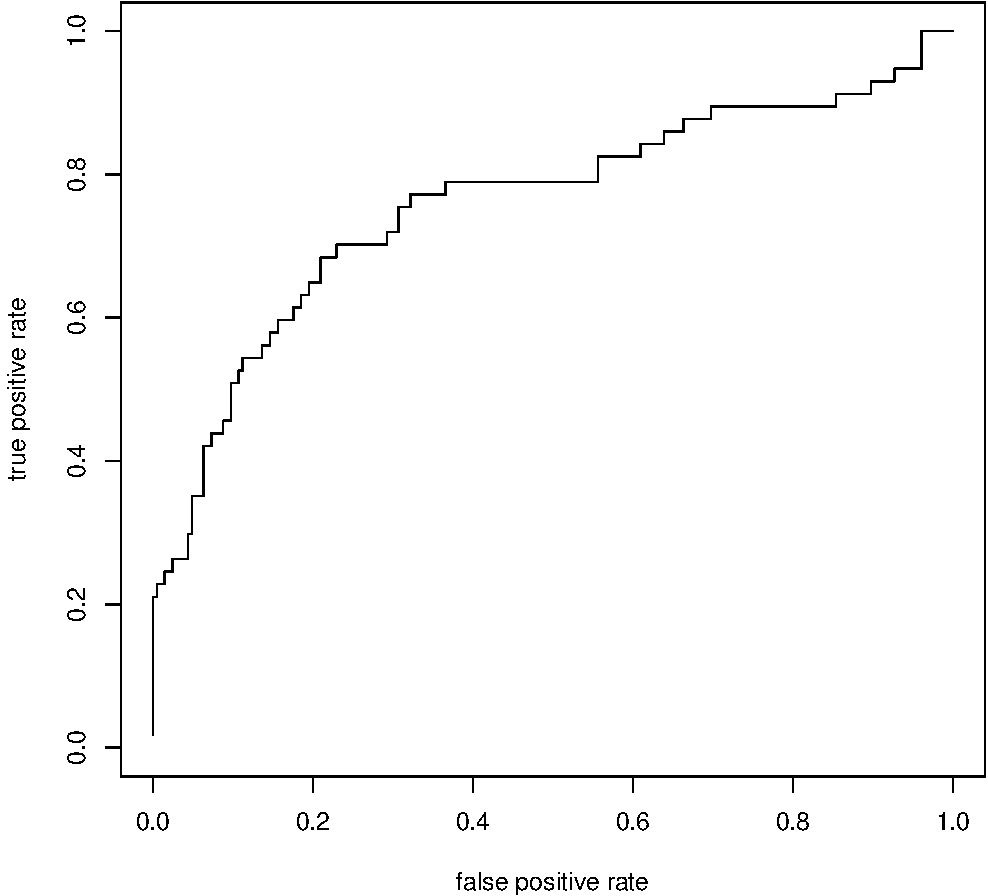
\includegraphics[width=\textwidth]{pic/ROC_DS1_1000_025.pdf}
\caption*{using data set \#0 \& \#1}
\end{minipage}
\begin{minipage}[b]{0.45\linewidth}
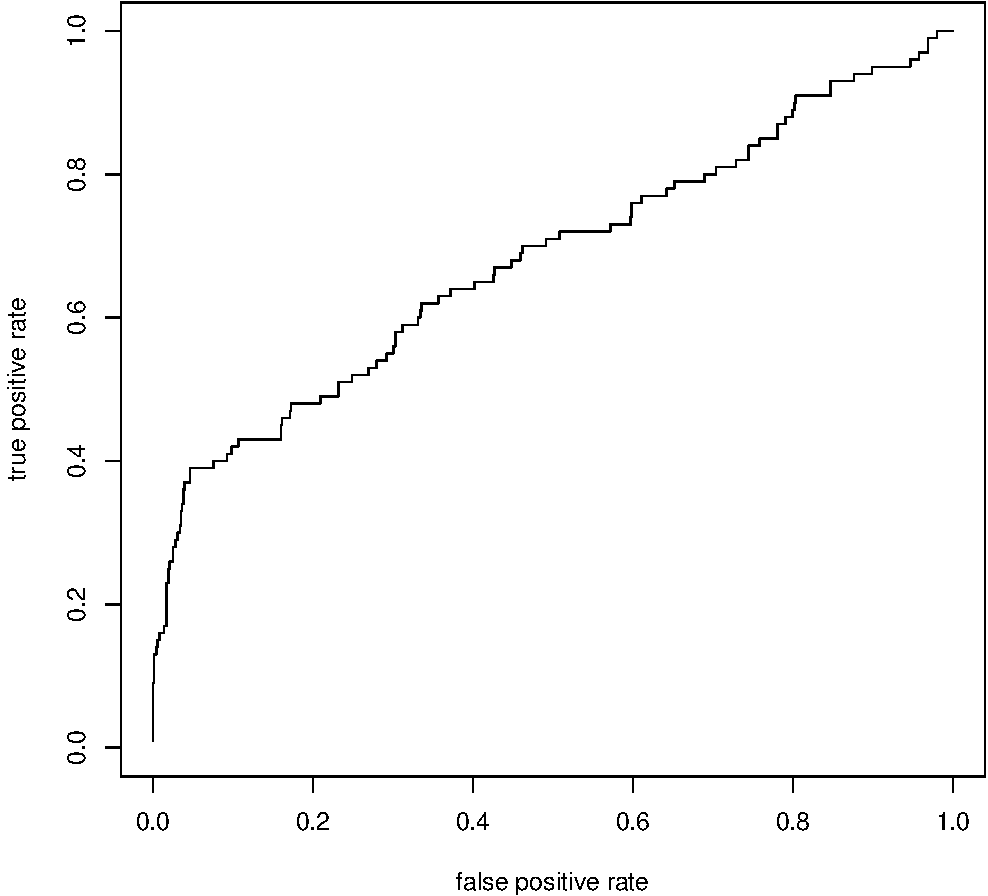
\includegraphics[width=\textwidth]{pic/ROC_DS2_1000_025.pdf}
\caption*{using data set \#0,\#1 \& \#2}
\end{minipage}
\caption{ ROC curve using leave-one-out cross validation}
\label{fig:ROC}
\end{figure}

In Figure \ref{fig:ROC}, note ROC curve to the left is better than the one to the right. This is because data set \#2 was generated by our algorithm based on the previous two data sets, and due to the exploration manner of our algorithm, data set \#2 should lie in the region that is more challenging for the classifier. Thus it is reasonable that our classifer performs worse using all available data sets. 

\subsection{Greedy Algorithm}
\subsubsection{Probability of Improvement}
We use equation \eqref{eq:PI3}, embeded in statistical model described in the previous section, to find peptides to sample next. 

Write equation \eqref{eq:model} as
\begin{equation} \label{model1}
\Prob\left(Y(x) = 1 | \theta\right) =
\frac{\prod_j \eta_j(x_j)}{\prod_j \eta_j(x_j) + \frac{\Prob(Y(x)=0)}{\Prob(Y(x)=1)}},
\end{equation}
where
\begin{equation*}
\eta_j(x_j) = \frac{\theta_{1,j}(x_j)}{\theta_{0,j}(x_j)} \text{\,\,\,for $\forall j \in \{1,\ldots,L\}$}. 
\end{equation*}
Then we can write equation \eqref{eq:PI3} as
\begin{equation} \label{eq:PI4}
\underset{e \in E \backslash S, f(e)<b}{\mathrm{arg}\max} \, \frac{\prod_j \eta_j(e_j)}{\prod_j \eta_j(e_j) + \frac{\Prob(Y(e)=0)}{\Prob(Y(e)=1)}},
\end{equation}
where 
\begin{equation*}
\eta_j(e_j)=\frac{\Prob(e_j|Y(e)=1,Y(x)=0, \forall x \in S)}{\Prob(e_j|Y(e)=0,Y(x)=0, \forall x \in S)}.
\end{equation*}
We can formulate equation \eqref{eq:PI4} as a Mixed-Integer Nonlinear Programming (MINLP),
\begin{equation} \label{eq:PI5}
\begin{split}
\max \quad &\frac{\prod_j \Sigma_k x_j(k) \eta_j(k)}{\prod_j \Sigma_k x_j(k) \eta_j(k) + \frac{\Prob(Y(x)=0)}{\Prob(Y(x)=1)}} \\
\text{s.t} \quad &k \in \{1,\ldots,K\} \\
&x_j(k) \in \{0,1\}\\
&\Sigma_k x_j(k)=1,
\end{split}
\end{equation}
where
\begin{equation*}
x_j(k)=\begin{dcases}
        1 & \text{if $e_j=k$}\\
        0 & \text{else}.
\end{dcases}
\end{equation*}
There are quite a few available software packages that can solve equation \eqref{eq:PI5} based on branch-and-bound. This is summarized in Algorithm \ref{algo1}.
\begin{Algorithm}(Probability of Improvement) \label{algo1}
\begin{algorithmic}[1]
\REQUIRE Inputs $\text{M, J, K}$, data set D and prior distribution of $\theta_y \sim \text{Dirichlet} (\boldsymbol \alpha_y), y \in \{1,0\}$
\STATE $S \leftarrow \emptyset $
\STATE Calculate posterior distribution of $\theta_1 \sim \text{Dirichlet} (\boldsymbol \alpha_1|\{x|x \in D,y(x)=1\})$.
\FOR{$m=1$ to $M$} 
\STATE COUNT $\leftarrow 0$
\STATE Calculate posterior distribution of $\theta_0 \sim \text{Dirichlet} (\boldsymbol \alpha_0|\{x|x \in D,y(x)=0\} \cup S)$.
\LOOP 
\STATE Sample $\theta_1$ from $\text{Dirichlet} (\boldsymbol \alpha_1|\{x|x \in D,y(x)=1\})$ and $\theta_0$ from $\text{Dirichlet} (\boldsymbol \alpha_0|\{x|x \in D,y(x)=0\} \cup S)$.
\STATE $\eta \leftarrow \frac{\theta_1}{\theta_0}$
\STATE Solve MINLP in equation \eqref{eq:PI5} to find $x$.
\STATE COUNT $\leftarrow$ COUNT $+ x$.
\ENDLOOP
\FOR {$j=1$ to $J$}
\STATE $e_j \leftarrow \underset{k \in \{1,\ldots,K\}}{\mathrm{arg}\max} \, \text{COUNT}_{kj}$
\ENDFOR
\STATE $S \leftarrow (S, e)$
\ENDFOR
\end{algorithmic}
\end{Algorithm}
We compare the performance of probability of improvement algorithm with two other methods: one method is to pick the most probable peptides based on posterior distribution, and the other is to randomly mutate known peptides $x$ such that $y(x)=1$ as our new recommendations. The benchmark was performed on a simulated dataset using the statistical model described in \ref{sec:stat model}, and we show the result in \ref{fig:PI}

% We use probability that shortest peptide $x$ with $y(x)=1$ has length smaller or equal to 12 as a measure of quality, to do the benchmark, and we show the result in Figure \ref{fig:PI}.
\begin{figure}[hpt] 
\center
\includegraphics[width=0.6\textwidth]{pic/to_add.pdf}
\caption{Benchmark of probability of improvement algorithm}
\label{fig:PI}
\end{figure}

\subsubsection{Expected Improvement}
Note that each term in the summation of \eqref{eq:EI1} has a similar structure as \eqref{eq:PI3}. Let $S=\{p^1,\ldots,p^{|S|}\}$, we can write \eqref{eq:EI1} as a MINLP:
\begin{equation} \label{eq:EI5}
\begin{split}
\max \quad &\Sigma_{i=0}^{|S|} c_i \frac{\prod_j \Sigma_k x_j(k) \eta_j^i(k)}{\prod_j \Sigma_k x_j(k) \eta_j^i(k) + \frac{\Prob(Y(x)=0)}{\Prob(Y(x)=1)}} (f_i-f(e))^+ \\
\text{s.t} \quad &k \in \{1,\ldots,K\} \\
&x_j(k) \in \{0,1\}\\
&\Sigma_k x_j(k)=1,
\end{split}
\end{equation}
where
\begin{equation*}
x_j(k)=\begin{dcases}
        1 & \text{if $e_j=k$}\\
        0 & \text{else},
\end{dcases}
\end{equation*}
\begin{equation*}
f_i=\begin{dcases}
        b & \text{if $i=0$}\\
        f(p^i)  & \text{else},
\end{dcases}
\end{equation*}
and $c_i$'s are known coefficients. We summarize it in Algorithm \ref{algo2}.

\begin{Algorithm}(Expected Improvement) \label{algo2}
\begin{algorithmic}[1]
\REQUIRE Inputs $\text{M, J, K}$, data set D and prior distribution of $\theta_y \sim \text{Dirichlet} (\boldsymbol \alpha_y), y \in \{1,0\}$
\STATE $S \leftarrow \emptyset $
\FOR{$m=1$ to $M$} 
\STATE COUNT $\leftarrow 0$
\IF{$S$ is not empty}
\STATE Sort elements in $S$ as $\{p^1,\ldots,p^{|S|}\}$ such that $f(p^i) \leq f(p^j), \forall i<j$.
\ENDIF
\STATE Calculate posterior distribution of $\theta_1^0 \sim \text{Dirichlet} (\boldsymbol \alpha_1|\{x|x \in D,y(x)=1\})$ and $\theta_0^0 \sim \text{Dirichlet} (\boldsymbol \alpha_0|\{x|x \in D,y(x)=0\} \cup S)$.
\FOR{$i=1$ to $|S|$}
\STATE Calculate posterior distribution of $\theta_1^i \sim \text{Dirichlet} (\boldsymbol \alpha_1|\{x|x \in D,y(x)=1\} \cup \{p^i\})$ and $\theta_0^i \sim \text{Dirichlet} (\boldsymbol \alpha_0|\{x|x \in D,y(x)=0\} \cup \{p^j|j<i\})$.
\ENDFOR
\LOOP 
\STATE Sample $\theta_1^{i=0:|S|}$ and $\theta_0^{i=0:|S|}$ from posterior distribution.
\STATE $\eta^{i=0:|S|} \leftarrow \frac{\theta_1^{i=0:|S|}}{\theta_0^{i=0:|S|}}$
\STATE Solve MINLP in equation \eqref{eq:EI5} to find $x$.
\STATE COUNT $\leftarrow$ COUNT $+ x$.
\ENDLOOP
\FOR {$j=1$ to $J$}
\STATE $e_j \leftarrow \underset{k \in \{1,\ldots,K\}}{\mathrm{arg}\max} \, \text{COUNT}_{kj}$
\ENDFOR
\STATE $S \leftarrow (S, e)$
\ENDFOR
\end{algorithmic}
\end{Algorithm}
Benchmark to be added here.

\subsection{Performance on real experiment data.}
Given the initial training data with size ?, we have performed two rounds of experiments using recommendations generated by Probability of Improvement algorithm. In the first round we performed experiments on 

\section{Conclusion}
We presented two greedy heuristic algorithms solving active learning problem described in \ref{sec:prob state}, and proved that both of these two algorithms guarantee to achieve at least a factor (1-1/e) of the optimal value. From benchmark results, we further showed that these two algorithms outperformed another two heuristic search methods. In addition to theoretic results, We demonstrated effectiveness of our methods by applying them to optimal experimental design problem in material science, in which we are searching for shortest peptides that act as a substrate for some specific enzymes. We developed a Naive Bayes classifier to model the problem, and used our algorithm to propose candidates for testing by experiment. From the preliminary testing result made by our experimental collaborator, we have found a few short peptides that are very likely to be substrate of target enzymes.

% Appendix here
% Options are (1) APPENDIX (with or without general title) or
%             (2) APPENDICES (if it has more than one unrelated sections)
% Outcomment the appropriate case if necessary
%
% \begin{APPENDIX}{<Title of the Appendix>}
% \end{APPENDIX}
%
%   or
%
% \begin{APPENDICES}
% \section{<Title of Section A>}
% \section{<Title of Section B>}
% etc
% \end{APPENDICES}

%%
% \theendnotes

% Acknowledgments here
% \ACKNOWLEDGMENT{The authors gratefully acknowledge the existence of
% the Journal of Irreproducible Results and the support of the Society
% for the Preservation of Inane Research.}


% References here (outcomment the appropriate case)

% CASE 1: BiBTeX used to constantly update the references
%   (while the paper is being written).
%\bibliographystyle{ormsv080} % outcomment this and next line in Case 1
%\bibliography{<your bib file(s)>} % if more than one, comma separated

% CASE 2: BiBTeX used to generate mypaper.bbl (to be further fine tuned)
%\input{mypaper.bbl} % outcomment this line in Case 2

%If you don't use BiBTex, you can manually itemize references as shown below.


\begin{thebibliography}{}

\bibitem[Chen et~al., 2013]{Chen2013}
Chen, Y., Krause, A., and Zurich, E. T.~H. (2013).
\newblock {Near-optimal Batch Mode Active Learning and Adaptive Submodular
  Optimization}.
\newblock 28.

\bibitem[Ginsbourger et~al., 2008]{Ginsbourger2008}
Ginsbourger, D., Riche, R.~L., and Carraro, L. (2008).
\newblock {A multi-points criterion for deterministic parallel global
  optimization based on Gaussian processes}.
\newblock {\em In Intl. Conf. on Nonconvex Programming, NCP07, page ..., Rouen,
  France.}, pages 1--30.

\bibitem[Hoi et~al., 2006a]{Hoi2006a}
Hoi, S. C.~H., Jin, R., and Lyu, M.~R. (2006a).
\newblock {Large-scale text categorization by batch mode active learning}.
\newblock {\em Proceedings of the 15th international conference on World Wide
  Web - WWW '06}, page 633.

\bibitem[Hoi et~al., 2006b]{Hoi2006}
Hoi, S. C.~H., Jin, R., Zhu, J., and Lyu, M.~R. (2006b).
\newblock {Batch mode active learning and its application to medical image
  classification}.
\newblock {\em Proceedings of the 23rd international conference on Machine
  learning - ICML '06}, pages 417--424.

\bibitem[Jones et~al., 1998]{Jones1998}
Jones, D., Schonlau, M., and Welch, W. (1998).
\newblock {Efficient global optimization of expensive black-box functions}.
\newblock {\em Journal of Global optimization}, pages 455--492.

\bibitem[Negoescu et~al., 2010]{Negoescu2010}
Negoescu, D.~M., Frazier, P.~I., and Powell, W.~B. (2010).
\newblock {The Knowledge-Gradient Algorithm for Sequencing Experiments in Drug
  Discovery}.
\newblock {\em INFORMS Journal on Computing}, 23(3):346--363.

\bibitem[NemHauser et~al., 1978]{Company1978}
NemHauser, G., Fisher, M., and Wolsey, L. (1978).
\newblock {An Analysis of Approximations for Maximizing Submodular Set
  Functions}.
\newblock 14:265--294.

\bibitem[{Feldman and Schwan(1990)}]{fs}
Feldman D, Schwan K (1990) {\it Who Put the Butter in Butterfly
and Other Fearless Investigations into Our Illogical Language}
(HarperPerennial, New York).

\bibitem[{Fontecha et~al.(2006)}]{fo}
Fontecha J, Mayo I, Toledano G, Juarez M (2006)
Triacylglycerol composition  of projected designation
of origin cheeses during ripening. {\it J. Dairy Sci.} 89:882--887.

\bibitem[{Geisel(1984)}]{g}
Geisel TS (1984) {\it The Butter Battle Book\/} (Random House, New York).

\bibitem[{Hodson et~al.(2001)}]{h}
Hodson L, Skeaff CM, Chisholm W-AH (2001) The effect of
replacing dietary saturated fat with polyunsaturated or
monounsaturated fat on plasma lipids in free-living young adults.
{\it Eur. J. Clinical Nutrition} 55(10):908--915.

\bibitem[{Tholstrup et al.(2006)}]{trbn} 
Tholstrup T, Raff M, Basu S, Nonboe P, Sejrsen K, Staarup EM (2006) 
Effects of butter and mono\-un\-saturated fatty acids
into lipid classes, plasma C-reactive protein, oxidative stress,
hemostatic variables, and insulin in healthy young men. {\it Amer. J.
Clinical Nutrition} 83:237--243.

\bibitem[{Torbica et al.(2006)}]{tjp}
Torbica A, Jovanovic O, Pajin B (2006) The advantages of solid
fat content determination in cocoa butter and cocoa butter
equivalents by the Karlshamns method. {\it Eur. Food Res. Techn.} 222:385--391.

\end{thebibliography}
%%%%%%%%%%%%%%%%%
\end{document}
%%%%%%%%%%%%%%%%%
